% !TEX root = ../main.tex
% called by main.tex
\chapter{Particularidades de la Impresión 3D}\label{ch:3d-intro}

\section{Proceso de fabricación}
Para fabricar piezas impresas en 3D, es necesario de alguna manera, hacer llegar la información de la pieza a la impresora. Estas ``instrucciones'' son un código \texttt{GCODE}. Este tipo de códigos son un estándar utilizado para el control de máquinas herramientas de control numérico, una forma algo pomposa de describir una impresora 3D, pero es que el \texttt{GCODE} es el mismo código que utilizan las fresas o tornos CNC o máquinas de mecanizado por control numérico multieje. 
\par La obtención de estos códigos \texttt{GCODE} es muy sencilla. El proceso lo explicaré secuencialmente partiendo desde el programa de diseño 3D, hasta el momento de dar la orden a la impresora de fabricar la pieza. 

\subsection{De un diseño a una pieza real}
Teniendo por fin el diseño terminado, este no es más que una colección de ecuaciones que describen la geometría de la pieza. Para fabricarla, \textbf{exportaremos} este diseño como un archivo \texttt{.stl} o \texttt{.step/.stp}. Este tipo de archivos son un conjunto de triángulos en el caso del \texttt{.stl}, o un conjunto de ecuaciones en el caso del \texttt{.step/.stp} (esta vez estandarizado para ser comprensible para cualquier otro programa) que describen la geometría de la pieza. 
\par Ahora tenemos un archivo que es fácilmente comprensible para cualquier programa, no solo nuestro programa de diseño. Ahora, abriremos nuestro Slicer. En el slicer, deberemos elegir la orientación y la posición de la pieza en la cama de la impresora, así como algunos parámetros adicionales. Una vez satisfechos, solamente hay que hacer click en \textbf{slice} y el programa nos enseñará una previsualización de cómo quedará la pieza, mostrando las pasadas individuales del cabezal de la impresora.
\par Este archivo \texttt{GCODE} contendrá todas las instrucciones para la impresora, la temperatura a la que deberá calentar el cabezal, la cama, a dónde se tendrá que mover para cada deposición de filamento, etc. No hace falta entender nada de esto a más bajo nivel, ni siquiera es importante entender qué quieren decir las líneas dentro del archivo, no hace falta mirar dentro. Simplemente este archivo lo pasaremos a la impresora, guardándolo en la tarjeta micro SD de la impresora.
\todo{Añadir imágenes de la impresora, la tarjeta  y el lector del ordenador}. 
\par Finalmente, al introducir la tarjeta de nuevo en la impresora y encenderla, podremos navegar por los menús hasta seleccionar nuestro archivo \texttt{GCODE}. Al seleccionarlo, la impresora comenzará a imprimir la pieza.

\section{Importancia del Slicer}
Como se puede observar, el Slicer es una de las herramientas más poderosas en la impresión 3D, y un buen resultado dependerá tanto del diseño de la pieza, su geometría, como del Slicer. Esto es porque el Slicer tiene en cuenta una infinidad de parámetros, como las dimensiones de la impresora, las velocidades a las que se moverá, qué filamento estamos imprimiendo, qué temperaturas se utilizarán para ese filamento, etc. 
\par Generalmente, se utilizará la configuración predeterminada y ajustada a nuestra impresora, y no habrá que cambiar mucho estos ajustes. Por otro lado, para conseguir piezas más rígidas o más resistentes, en muchas ocasiones es suficiente con cambiar ajustes del Slicer y no es necesario rediseñar la geometría de la pieza. 
\par Es importante recalcar que con la experiencia y el uso, hemos conseguido encontrar en el club de vuelo una serie de ajustes para el Slicer que nos permiten conseguir impresiones rápidas, de una resistencia más que suficiente y con un nivel de detalles perfectamente adecuado para todos nuestros diseños. Por otro lado, si una pieza requiere una configuración muy particular de los ajustes del Slicer, el diseño de la propia pieza se deberá hacer con todo esto en cuenta. 

\section{Anisotropía de las piezas}
Por la propia naturaleza de la impresión 3D, es importante considerar cuál será el funcionamiento de las piezas, y a qué tipo de esfuerzos estarán sometidas. Esto nos permitirá elegir en qué orientación sería preferente imprimirlas. 

\par Debemos tener en cuenta que las piezas son mucho más susceptibles a romper bajo esfuerzos de tracción o pelado perpendiculares a los planos de las capas. Por ello hay que elegir una orientación que coloque los esfuerzos de tracción en el plano de las capas, como se puede observar en la \autoref{fig:fallo-traccion}. Sin embargo, las piezas impresas en 3D  funcionan mejor a compresión perpendicular al plano de las capas que en el plano. 

\begin{figure}[ht]
    \centering
    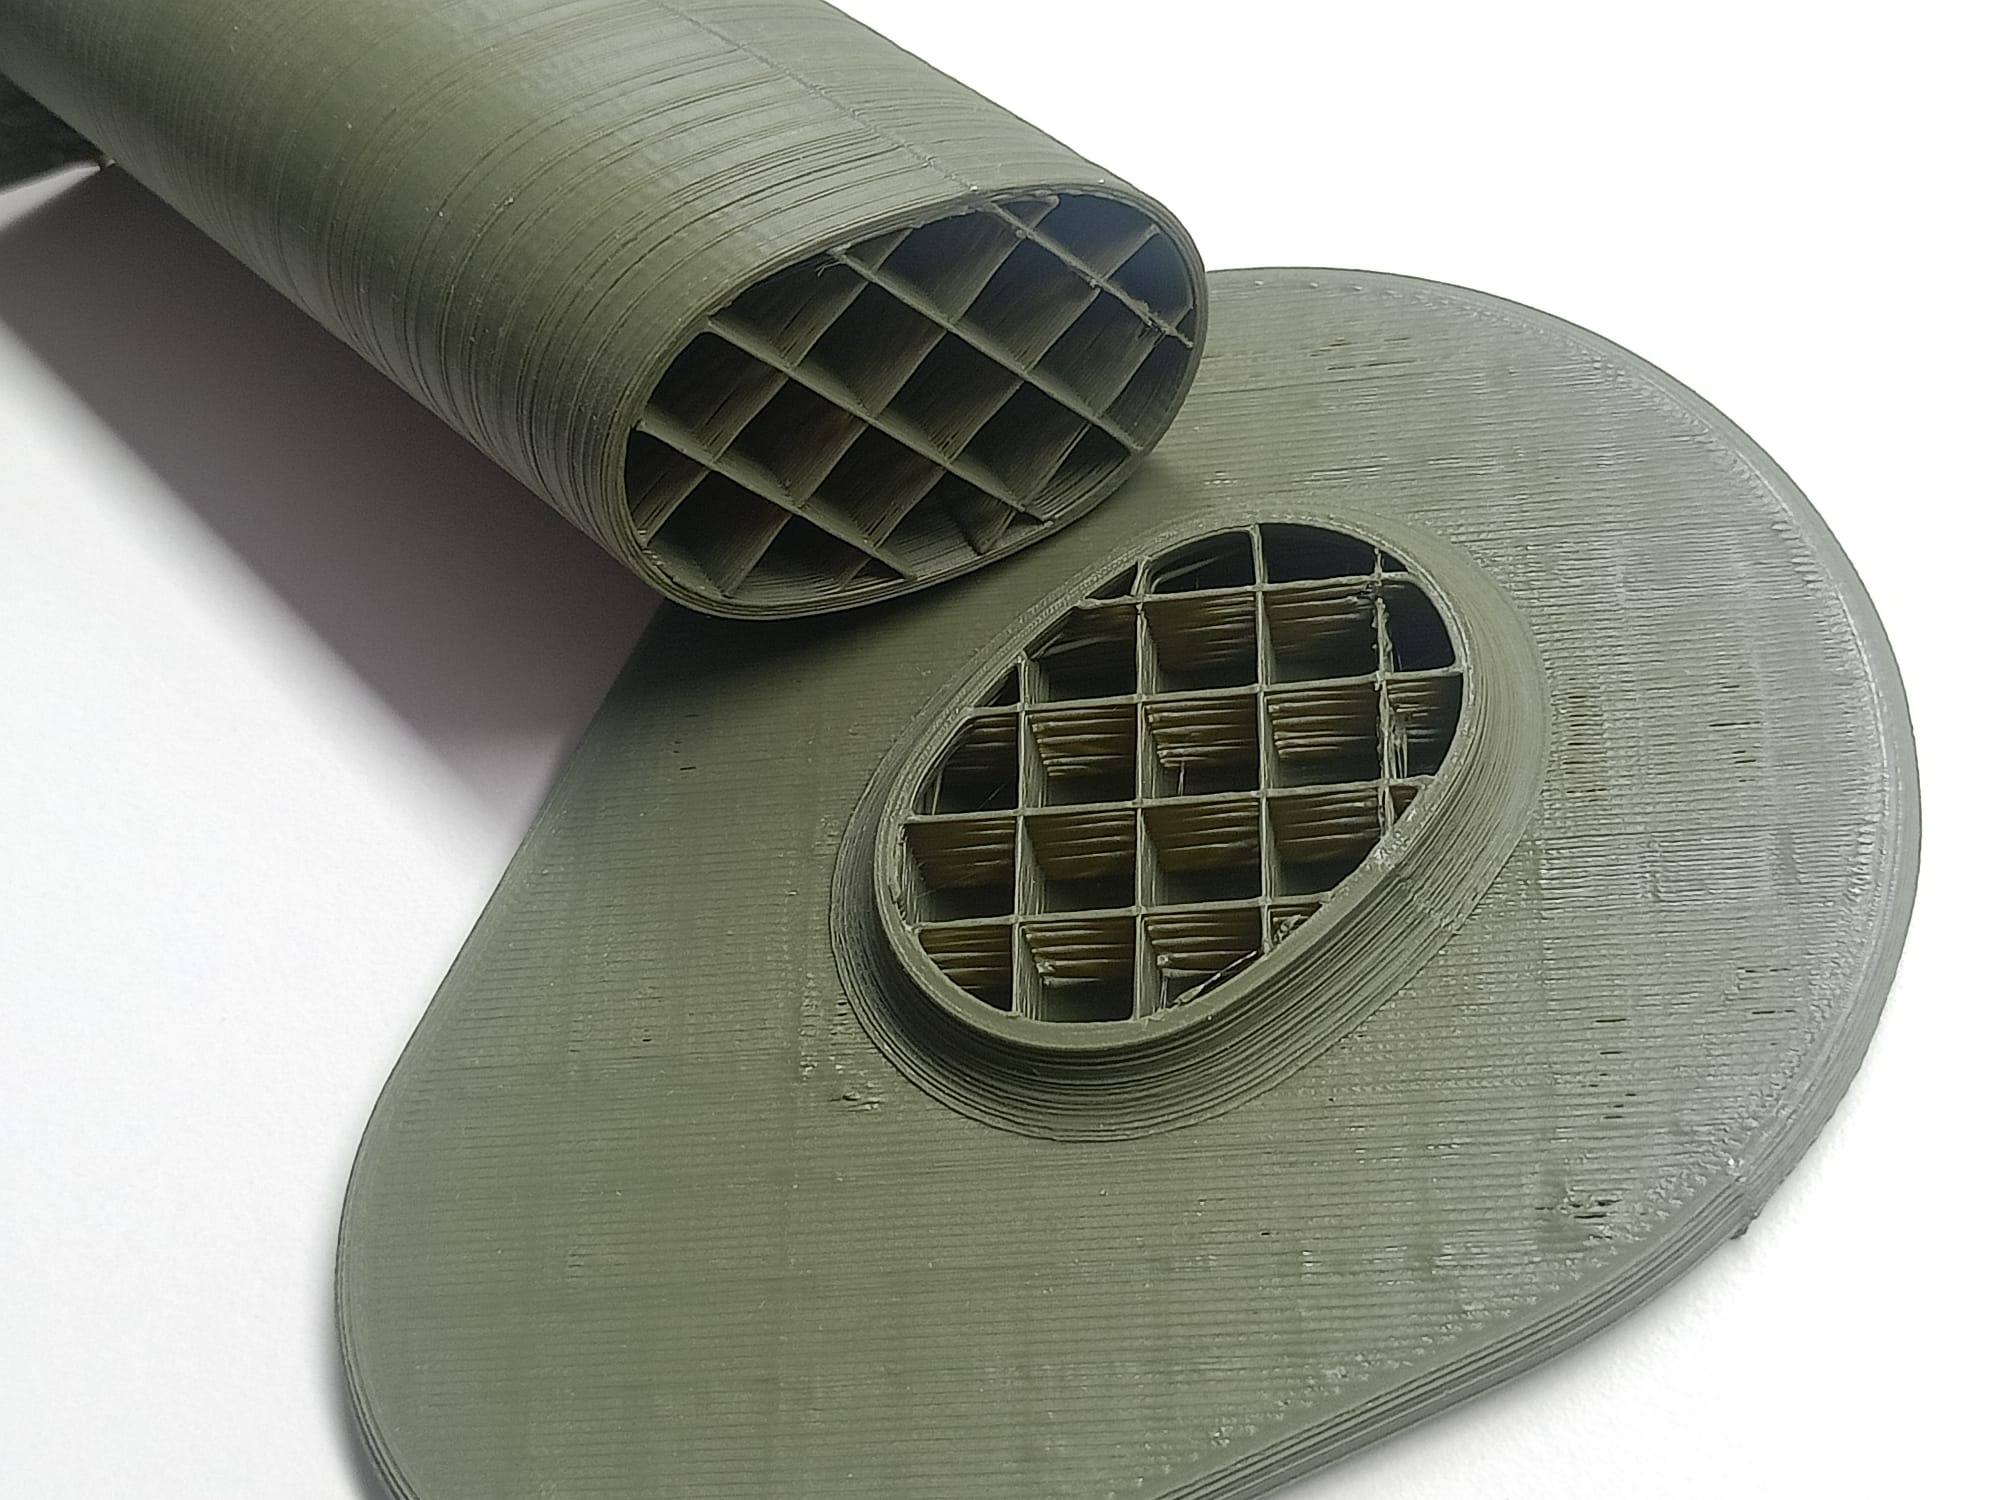
\includegraphics[width=0.5\textwidth]{figures/fallo-traccion.jpg}
    \caption{Ejemplo de un fallo por tracción en la dirección perpendicular a las capas}
    \label{fig:fallo-traccion}
\end{figure}
\todo{Añadir más imágenes de fallos en piezas impresas}

\section{Enfriamiento de las piezas}
Otro de los factores que más pueden conducir a error es no considerar, en piezas con cambios muy importantes en la sección, el enfriamiento desigual de la pieza.
\par El filamento es calentado hasta a unos 200\textdegree{}C típicamente para ser impreso, e inmediatamente después es enfriado hasta su temperatura de transición vítrea ($\approx 180$\textdegree{}C) al salir por la boquilla de la impresora. Una vez ha sido depositado, continúa enfriándose lentamente hasta la temperatura del resto de la pieza, que serán unos 60\textdegree{}C. Los gradientes térmicos que se presentan en estas situaciones son muy significativos, y el plástico experimentará expansiones y sobre todo, contracciones térmicas al ir reduciendo su temperatura. 
\par El enfriamiento genera esfuerzos internos en la pieza, generarán tracción en la dirección en la que el filamento haya sido depositado, pudiendo llegar a combar las piezas planas si la adherencia a la cama de la impresora no es suficiente.
\par Este tipo de problemas está agravado por el hecho de que la adherencia del PETG al vidrio (el material con el que más se imprime en el Club de Vuelo y el material de la cama de nuestra impresora) es muy baja. Es por esto que es tan importante utilizar la laca de la impresora generosamente, o conseguir un fleje metálico y texturizado para colocar en la cama. 